% one-figure manuscript written by fig_qc.py --tek-sekil-tex (trap T29)
\begin{figure*}[!t]
\centering
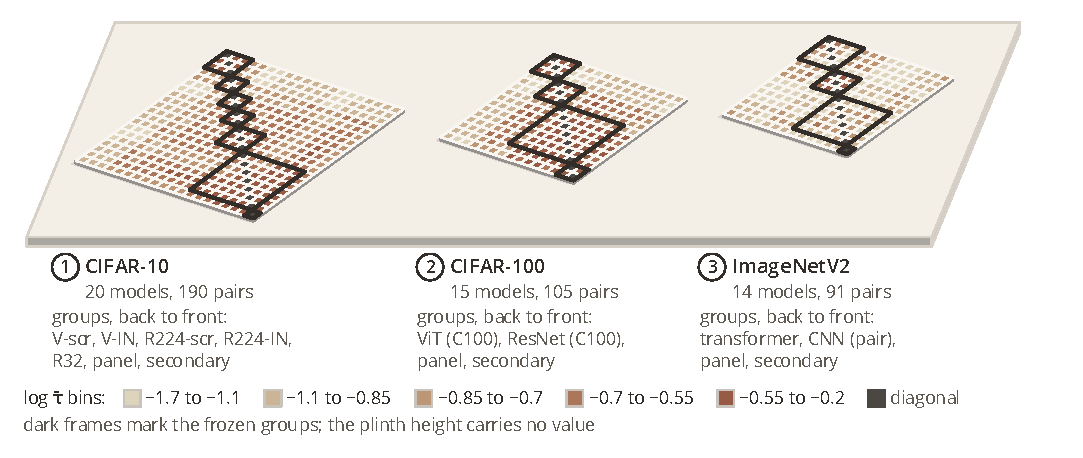
\includegraphics{fig8_similarity_matrix}
\caption{\textbf{Pairwise symmetric similarity.} log τ̄ (split-half) for all models on CIFAR-10 (1), CIFAR-100 (2) and ImageNetV2 (3), rows and columns in frozen group order; cell colour is one of five joint quintile bins, the dark diagonal undefined, dark frames mark the groups. Scratch-trained ViT-Tiny seeds form a block dissimilar to the CNN panel.}
\label{fig:fig8_similarity_matrix}
\end{figure*}
